
%(BEGIN_QUESTION)
% Copyright 2014, Tony R. Kuphaldt, released under the Creative Commons Attribution License (v 1.0)
% This means you may do almost anything with this work of mine, so long as you give me proper credit

En av motstandene i denne spenningsdeleren har feil (enten åpen eller kortsluttet). Basert på spenningsmålingene ved hver last, avgjør hvilken motstand det er og hvilken feiltype den har:

$$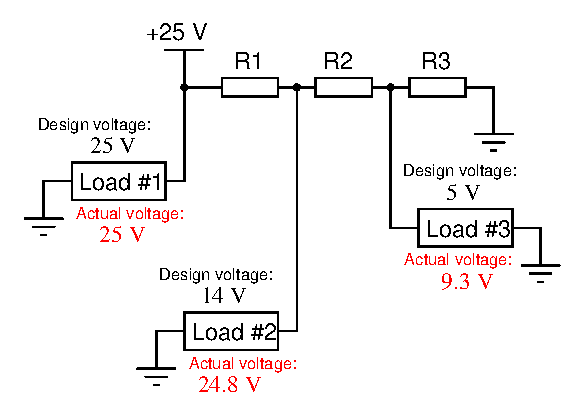
\includegraphics[width=15.5cm]{i01136x01.eps}$$

\underbar{file i01136}
%(END_QUESTION)





%(BEGIN_ANSWER)

Motstand R1 har feil og er (delvis) kortsluttet. Det ser vi fordi både last \#2 og \#3 overbelastes.

%(END_ANSWER)





%(BEGIN_NOTES)

Diskuter med elevene hvordan de kunne forutsi at R1 var feilmotstanden. Finnes det noen tydelig ledetråd i diagrammet som peker på R1?  Noen elever kan mistenke at en åpen feil i R3 kan gi samme symptomer, men det finnes en tydelig måte å se at problemet {\it kun} kan skyldes en kortslutning i R1 (hint: analyser R2). 

Forklar at ikke alle ``kortsluttede'' feil er ``harde'' i betydningen direkte metall-mot-metall-forbindelse. Ofte feiler komponenter kortsluttet i en ``mykere'' forstand, det vil si at de fortsatt har en ikke ubetydelig elektrisk resistans.

%INDEX% Elektronikkrepetisjon: serie-parallellkretser

%(END_NOTES)


